% !TEX TS-program = pdflatex
% !TEX encoding = UTF-8 Unicode

% This file is a template using the "beamer" package to create slides for a talk or presentation
% - Giving a talk on some subject.
% - The talk is between 15min and 45min long.
% - Style is ornate.

% MODIFIED by Jonathan Kew, 2008-07-06
% The header comments and encoding in this file were modified for inclusion with TeXworks.
% The content is otherwise unchanged from the original distributed with the beamer package.

\documentclass{beamer}


% Copyright 2004 by Till Tantau <tantau@users.sourceforge.net>.
%
% In principle, this file can be redistributed and/or modified under
% the terms of the GNU Public License, version 2.
%
% However, this file is supposed to be a template to be modified
% for your own needs. For this reason, if you use this file as a
% template and not specifically distribute it as part of a another
% package/program, I grant the extra permission to freely copy and
% modify this file as you see fit and even to delete this copyright
% notice. 


\mode<presentation>
{
  \usetheme{Warsaw}
  % or ...

  \setbeamercovered{transparent}
  % or whatever (possibly just delete it)
}

\usepackage{tikz}
\usepackage{graphicx}
\usepackage[english]{babel}
% or whatever

\usepackage[utf8]{inputenc}
% or whatever

\usepackage{times}
\usepackage[T1]{fontenc}
% Or whatever. Note that the encoding and the font should match. If T1
% does not look nice, try deleting the line with the fontenc.


\title[Short Paper Title] % (optional, use only with long paper titles)
{Practical Steps for Increasing Openness and Reproducibility}

\subtitle
{Discussion} % (optional)

\author[Christensen] % (optional, use only with lots of authors)
{Garret Christensen\inst{1}}
% - Use the \inst{?} command only if the authors have different
%   affiliation.

\institute[UC Berkeley, Berkely Initiatiative for Transparency in the Social Sciences] % (optional, but mostly needed)
{
  \inst{1}%
  UC Berkeley: Berkely Initiatiative for Transparency in the Social Sciences\\
  Center for Open Science
}
% - Use the \inst command only if there are several affiliations.
% - Keep it simple, no one is interested in your street address.

\date[Short Occasion] % (optional)
{April 24, 2015 UC Riverside}

\subject{Talks}
% This is only inserted into the PDF information catalog. Can be left
% out. 


% Delete this, if you do not want the table of contents to pop up at
% the beginning of each subsection:
%\AtBeginSubsection[]
%{
%  \begin{frame}<beamer>{Outline}
%   \tableofcontents[currentsection,currentsubsection]
%  \end{frame}
%}


% If you wish to uncover everything in a step-wise fashion, uncomment
% the following command: 

%\beamerdefaultoverlayspecification{<+->}

\begin{document}

% Since this a solution template for a generic talk, very little can
% be said about how it should be structured. However, the talk length
% of between 15min and 45min and the theme suggest that you stick to
% the following rules:  

% - Exactly two or three sections (other than the summary).
% - At *most* three subsections per section.
% - Talk about 30s to 2min per frame. So there should be between about
%   15 and 30 frames, all told.

\begin{frame}
  \titlepage
\end{frame}

\begin{frame}

\includegraphics[height=0.75in]{BITSSlogo.PNG}

 \url{bitss.org}
 
\includegraphics[height=0.75in]{COS.PNG}

\url{centerforopenscience.org}
\end{frame}

\begin{frame}{Outline}
  \tableofcontents
  % You might wish to add the option [pausesections]
\end{frame}


\section{Introduction}
\begin{frame}{Reproducibility \& Transparency}
\begin{itemize}
\item What are problems associated with reproducibility?
\item What are solutions to these problems?
\item What are practical tools to implement these solutions?
\end{itemize}
\end{frame}
%%%%%%%%%%%%%%%%%%%%%%%%%%%%%%%%%%%%%%%%%%%%%%%%%%%%%%%%%%%%%%%%%%
\section{Problems}
\begin{frame}{Problems}
 \begin{itemize}
 \item Publication bias
 \item Specification Searching
 \item Data not available
 \item Code not available/unintelligible
 \end{itemize}
\end{frame}

\subsection{Publication Bias}
 \begin{frame}{Publication Bias}
  \begin{itemize}
  \item
  Only signficant results get published, even though the null result might be the truth, so we can't distinguish the truly significant from the 5\% we should expect due to randomness.
  
  \item
  See \href{http://www.nejm.org/doi/full/10.1056/NEJMsa065779}{Turner et al. 2008} for medicine or \href{http://www.sciencemag.org/content/345/6203/1502}{Franco et al. 2014} for social sciences. 
 \end{itemize}
 \end{frame}
 
{ % all template changes are local to this group.
    \setbeamertemplate{navigation symbols}{}
    \begin{frame}[plain]
        \begin{tikzpicture}[remember picture,overlay]
            \node[at=(current page.center)] {
                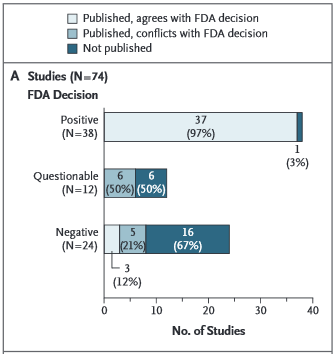
\includegraphics[height=\paperheight]{TurnerFigure1.PNG}
            };
        \end{tikzpicture}
     \end{frame}
}

\subsection{Specification Searching}
 \begin{frame}{Specification Searching}
  \begin{itemize}
  \item
  AKA Data mining, data dredging, p-hacking, fishing.
  
  \item
  Flexibility in analytical decisions lets you display practically anything as statistically significant. \href{http://pss.sagepub.com/content/22/11/1359}{Simmons, Nelson, Simonsohn (2011)} `proves' that listening to the Beatles makes you younger.
  \end{itemize}
 \end{frame}
 
\subsection{Irreproducible Workflow}
 \begin{frame}{Irreproducible Workflow}
 \begin{itemize}
 \item
  Even with the original authors' help, you can't get the data to reproduce the published results. Or you just can't find the data to begin with. 
  \item \textit{Journal of Money, Credit, and Banking} Project. \href{http://www.jstor.org/stable/1806061}{(Dewald et al., AER 1986)}
   \item Martin Feldstein on Social Security and private savings, Reinhart and Rogoff on debt and GDP growth.
 \end{itemize} 
 \end{frame}
%%%%%%%%%%%%%%%%%%%%%%%%%%%%%%%%%%%%%%%%%%%%%%%%%%%%%%%%%%%%%%%%%%%%

\section{Solutions}
\begin{frame}{Solutions}
\begin{itemize}[<+->]
\item Study Registry
\item Pre-Analysis Plan
\item Reproducible Workflow
 \begin{itemize}
 \item Literate Programing 
 \item Data Sharing
 \end{itemize}
\end{itemize}
\end{frame}

%%%%%%%%%%%%%%%%%%%%%%%%%%%%%%%%%%%%%%%%%%%%%%%%%%%%%%%%%%%%%%%%%%%%%
\section{Tools}
\subsection{Registries}
\begin{frame}{Specific Tools}
\begin{itemize}[<+->]
\item Study Registry
\begin{itemize}
 \item \href{http://clinicaltrials.gov}{NIH's Clinical Trial Registry}
 \item \href{http://www.socialscienceregistry.org}{AEA Social Science Registry}
 \item \href{http://e-gap.org/design-registration}{Experiments in Governance and Politics (EGAP)}
 \item \href{http://ridie.3ieimpact.org/}{Registry for International Development Impact Evaluations (RIDIE)}
 \item \href{http://osf.io}{Open Science Framework (OSF) \beamergotobutton{Link}}
\end{itemize}
\end{itemize}
\end{frame}

\subsection{Pre-Analysis Plan}
\begin{frame}{Pre-Analysis Plan}
What is a PAP?
\begin{itemize}
\item
From 3ie: ``A pre-analysis plan is a detailed description of the analysis to be conducted that is written in advance of seeing the data on impacts of the program being evaluated. It may specify hypotheses to be tested, variable construction, equations to be estimated, controls to be used, and other aspects of the analysis. A key function of the pre-analysis plan is to increase transparency in the research. By setting out the details in advance of what will be done and before knowing the results, the plan guards against data mining and specification searching. Researchers are encouraged to develop and upload such a plan with their study registration, but it is not required for registration.''
\end{itemize}
\end{frame}

\begin{frame}{Origin: FDA's Guidance for Industry}
``E9 Statistical Principles for Clinical Trials'' (1998)
\href{http://www.fda.gov/downloads/drugs/guidancecomplianceregulatoryinformation/guidances/ucm073137.pdf}{\beamergotobutton{Link}}

\S V Data Analysis Considerations
\begin{enumerate}
\item Prespecification of the Analysis
\item Analysis Sets
\item Missing Values and Outliers
\item Data Transformation
\item Estimation, Confidence Intervals, and Hypothesis Testing
\item Adjustment of Significance and Confidence Levels
\item Subgroups, Interactions, and Covariates
\item Integrity of Data and Computer Software Validity
\end{enumerate}
\end{frame}


\begin{frame}{Glennerster, Takavarasha Suggestions}
\textit{Running Randomized Evaluations}
\begin{enumerate}[<.->]
\def\labelenumi{\arabic{enumi}.}
\item
  the main outcome measures,
\item
  which outcome measures are primary and which are secondary,
\item
  the precise composition of any families that will be used for mean
  effects analysis,
  \begin{itemize}
  \item Mean effects: FWER, FDR using \href{http://dx.doi.org/10.1198/016214508000000841}{Anderson (JASA 2008)}.
  \end{itemize}
\item
  the subgroups that will be analyzed,
\item
  the direction of expected impact if we want to use a one-sided test,
  and
\item
  the primary specification to be used for the analysis.
\end{enumerate}
\end{frame}

\begin{frame}{McKenzie Suggestions}
\href{http://blogs.worldbank.org/impactevaluations/a-pre-analysis-plan-checklist}{World Bank Development Impact Blog}

\begin{enumerate}[<.->]
\item
  Description of the sample to be used in the study
\item
  Key data sources
\item
  Hypotheses to be tested throughout the causal chain
\item
  Specify how variables will be constructed
\item
  Specify the treatment effect equation to be estimated
\item
  What is the plan for how to deal with multiple outcomes and multiple
  hypothesis testing?
\item
  Procedures to be used for addressing survey attrition
\item
  How will the study deal with outcomes with limited variation?
\item
  If you are going to be testing a model, include the model
\item
  Remember to archive it
\end{enumerate}
\end{frame}

\subsection{Workflow}
\begin{frame}{Reproducible Workflow}
 \begin{itemize}
 \item R Markdown and \href{http://rstudio.com}{R Studio} to write dynamic documents.
 \item Version control with \href{http://www.github.com}{Github} or \href{http://osf.io}{OSF}. 
 \item Literate Programing
  \begin{itemize}
   \item Writing code to be read by a human instead of a machine. (Loosely: commenting the hell out of it.)
  \end{itemize} 
 \item Data Sharing
 \begin{itemize}
 \item \href{http://www.thedata.org}{Harvard's Dataverse}
 \end{itemize}
\end{itemize}
\end{frame}

{ % all template changes are local to this group.
    \setbeamertemplate{navigation symbols}{}
    \begin{frame}[plain]
        \begin{tikzpicture}[remember picture,overlay]
            \node[at=(current page.center)] {
                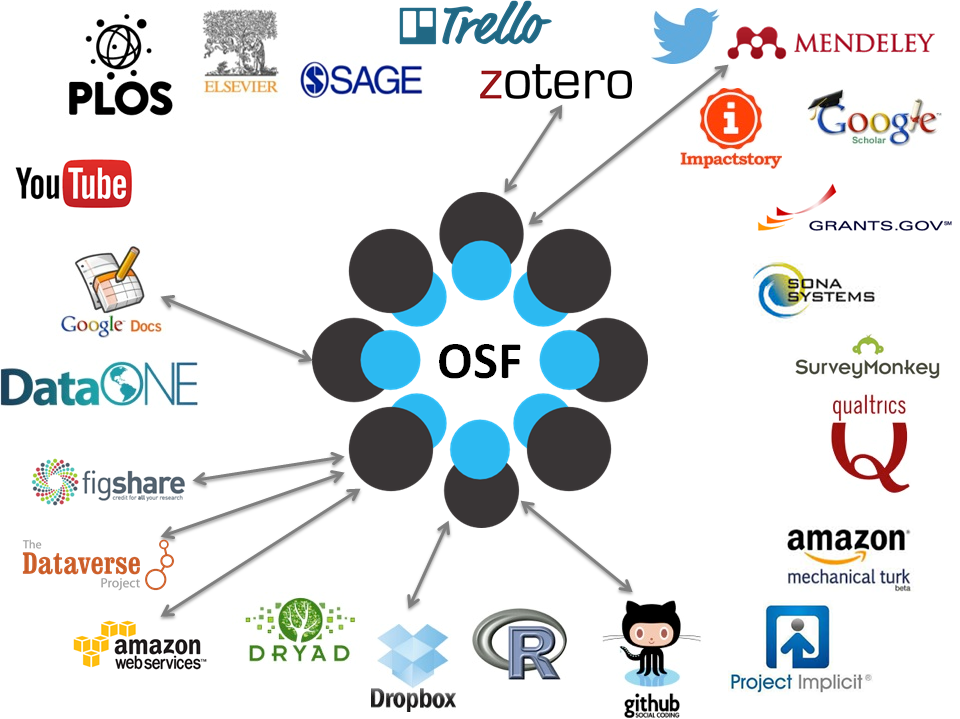
\includegraphics[height=\paperheight]{OSFnow.PNG}
            };
        \end{tikzpicture}
     \end{frame}
 % all template changes are local to this group.
    \setbeamertemplate{navigation symbols}{}
    \begin{frame}[plain]
        \begin{tikzpicture}[remember picture,overlay]
            \node[at=(current page.center)] {
                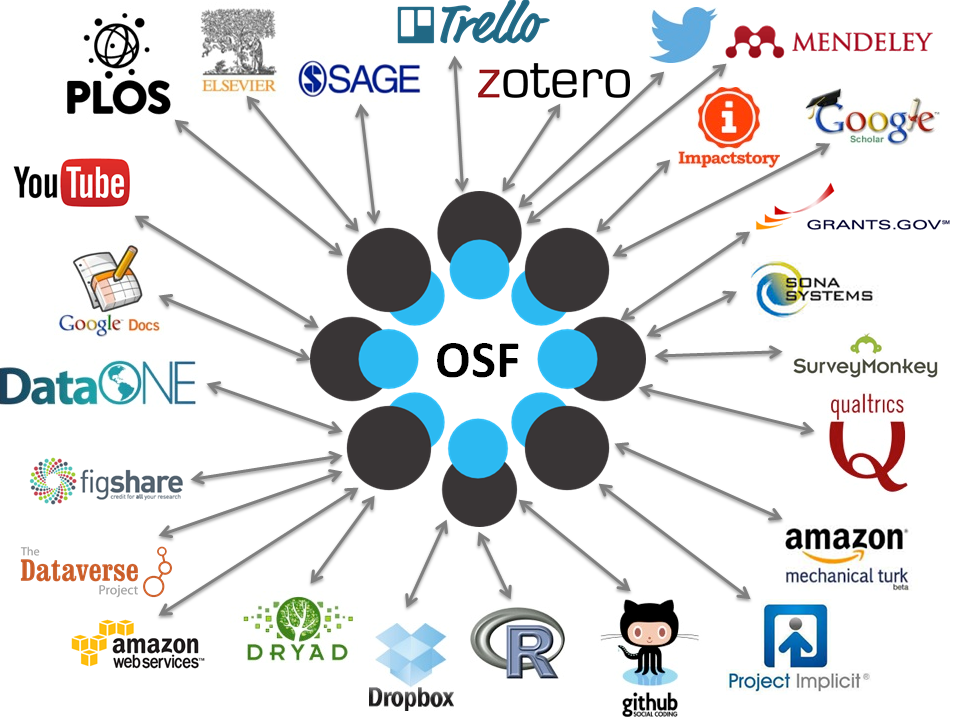
\includegraphics[height=\paperheight]{OSFsoon.PNG}
            };
        \end{tikzpicture}
     \end{frame}
}

\section{Conclusion}
\begin{frame}{Conclusion}
Simple tools exist to help you transparently and reproducibly take your research from beginning to end. 
\begin {itemize}
\item Open Science Framework
\item Trial Registries
\item Version Control
\item Dynamic Documents
\item Trusted Public Data Archive
\end{itemize} 
\vspace{0.25in}
Read more in my \href{http://github.com/garretchristensen/manual}{\textit{Manual of Best Practices in Transparent Social Science Research}} on GitHub.
\end{frame}


\end{document}


